\documentclass[12pt,compress,ngerman,utf8,t]{beamer}
\usepackage{etex}
\usepackage[ngerman]{babel}
\usepackage{calc,dashrule,tabto,tikz}
\usetikzlibrary{arrows}
\usepackage[protrusion=true,expansion=true]{microtype}
\usepackage[normalem]{ulem}

\graphicspath{{images/}}

\title[Unendlich große Zahlen]{\bf Die wundersame Welt der \\ unendlich großen Zahlen
\\[0.5em] \normalsize Glaube in der Mathematik?}
\author[Ingo Blechschmidt]{\textcolor{white}{Die Lange Nacht der Wissenschaft
\\ 16. Juli 2022}}
\date[2022-07-16]{\vspace*{5.5em}\ \\\textcolor{white}{Ingo Blechschmidt \\ \scriptsize
Lehrstuhl für Algebra und Zahlentheorie \\ Universität Augsburg \\}}

\useinnertheme[shadow=true]{rounded}
\useoutertheme{split}
\usecolortheme{orchid}
\usecolortheme{whale}
\setbeamerfont{block title}{size={}}

\useinnertheme{rectangles}

\usecolortheme{seahorse}
\definecolor{mypurple}{RGB}{150,0,255}
\setbeamercolor{structure}{fg=mypurple}
\definecolor{myred}{RGB}{150,0,0}
\setbeamercolor*{title}{fg=white}
\setbeamercolor*{titlelike}{bg=myred,fg=white}

\usefonttheme{serif}
\usepackage[T1]{fontenc}
\usepackage{libertine}

\setbeamertemplate{navigation symbols}{}

\setbeamertemplate{title page}[default][colsep=-1bp,rounded=false,shadow=false]
\setbeamertemplate{frametitle}[default][colsep=-2bp,rounded=false,shadow=false,center]

\newcommand{\hil}[1]{{\usebeamercolor[fg]{item}{\textbf{#1}}}}
\setbeamertemplate{frametitle}{%
  \vskip1em%
  \leavevmode%
  \begin{beamercolorbox}[dp=1ex,center]{}%
      \usebeamercolor[fg]{item}{\textbf{\textsf{\Large \insertframetitle}}}
  \end{beamercolorbox}%
}

\setbeamertemplate{footline}{%
  \leavevmode%
  \hfill%
  \begin{beamercolorbox}[ht=2.25ex,dp=1ex,right]{}%
    \usebeamerfont{date in head/foot}
    \insertframenumber\,/\,\inserttotalframenumber\hspace*{1ex}
  \end{beamercolorbox}%
  \vskip0pt%
}

\begin{document}

\addtocounter{framenumber}{-1}
{\usebackgroundtemplate{\includegraphics[width=\paperwidth]{infinity-space}}
\frame{\vspace*{-1em}\titlepage}}

\addtocounter{framenumber}{-1}
\begin{frame}{Fragen sind willkommen}
  \centering
  \includegraphics[width=0.70\textwidth]{conference-drew2018}

  Fragen sind während des gesamten Vortrags willkommen. \\
  Bitte keinesfalls bis zum Ende aufsparen. \\
  Vielen Dank dafür!
  \par
\end{frame}


\addtocounter{section}{-1}
\section{Große Zahlen}

{\usebackgroundtemplate{\begin{minipage}{\paperwidth}\vspace*{0cm}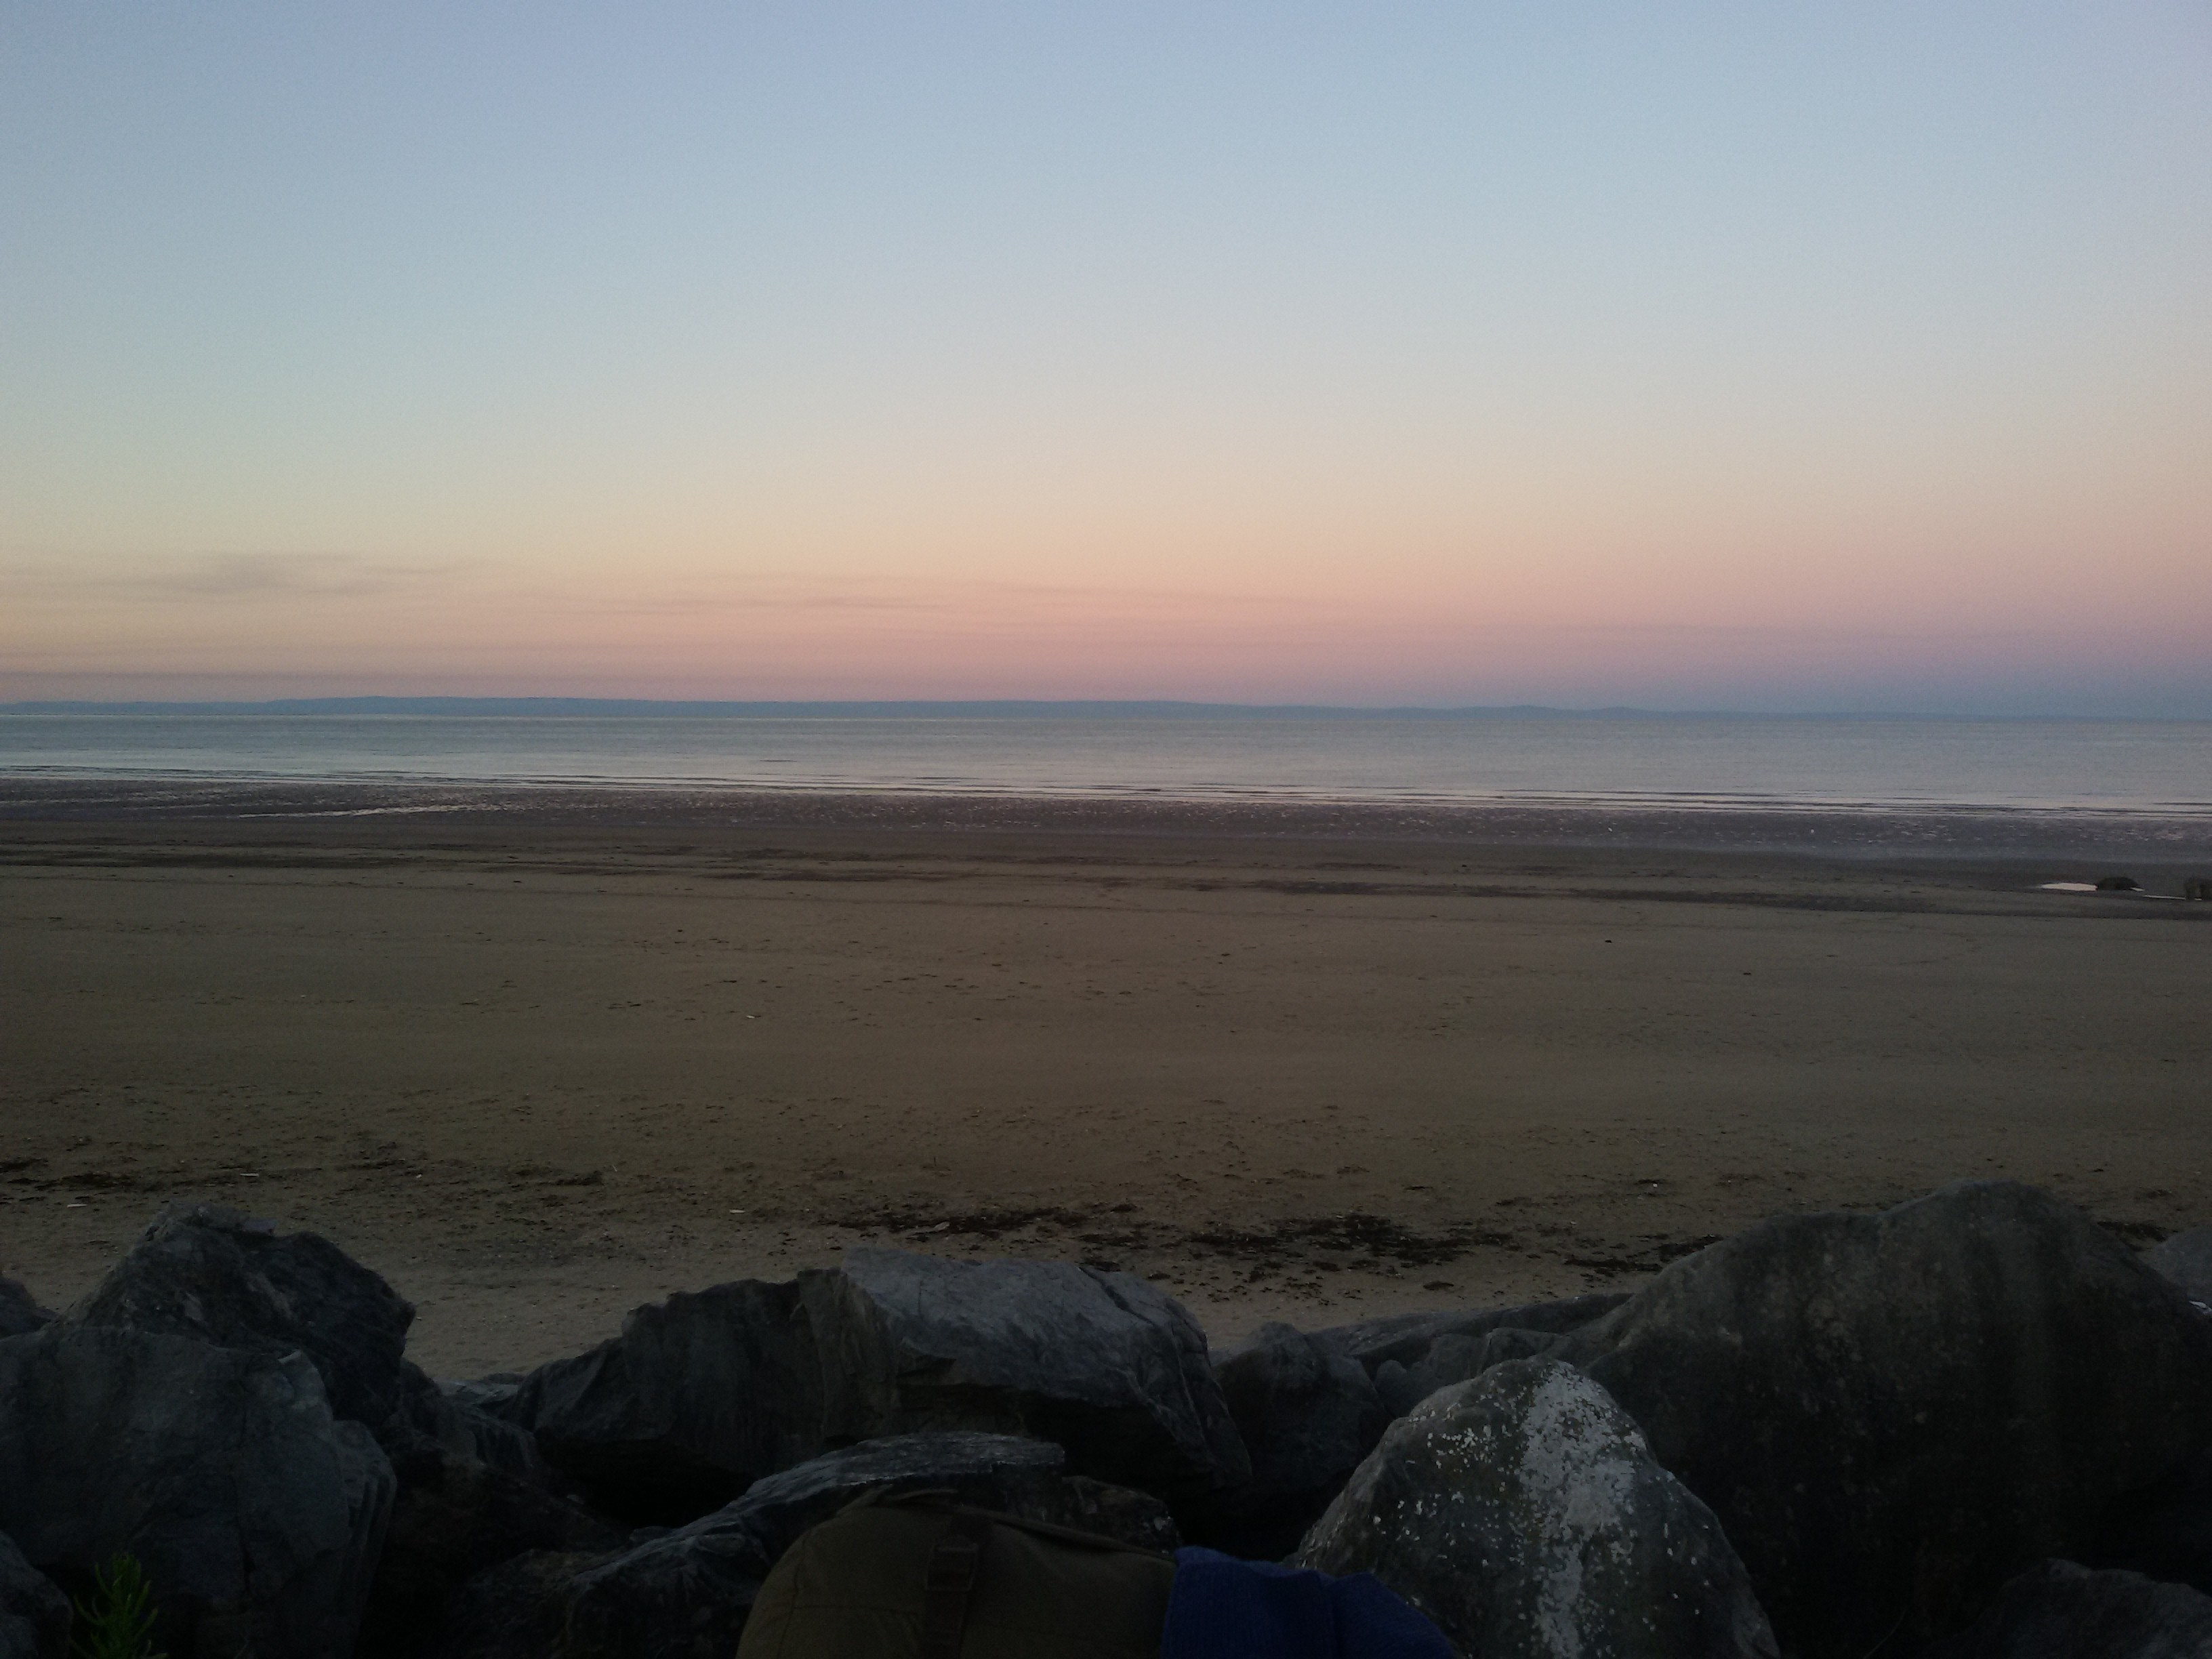
\includegraphics[width=\paperwidth]{swansea-bay}\end{minipage}}
\begin{frame}
  \centering
  \bigskip

  \Huge \hil{Teil 0}

  \bigskip
  \Large\textbf{Große Zahlen}
  \par
  \bigskip
  \bigskip
  \bigskip
  \bigskip
  \bigskip

  \normalsize
  \color{white}

  \hil{\color{white}300\,000} Augsburger*innen
  \pause
  \bigskip

  \hil{\color{white}$\boldsymbol{10^{19} = 1\!\underbrace{0\,000\,000\,000\,000\,000\,000}_{\text{$19$ Nullen}}}$}
  Sandkörner auf der Erde
  \pause
  \bigskip

  \hil{\color{white}$\boldsymbol{10^{80} = 1\!\underbrace{000\ldots000}_{\text{$80$ Nullen}}}$}
  Elementarteilchen im Universum
  \par
\end{frame}}

\newcommand{\imgslideHeight}[2]{{\usebackgroundtemplate{\parbox[c][\paperheight][c]{\paperwidth}{\centering\includegraphics[height=\paperheight]{#1}}}\begin{frame}[plain]\vspace*{17em}\pause\centering\bf\color{white}#2\end{frame}}}
\imgslideHeight{milky-way}{\vspace*{3em}$\boldsymbol{6\,000}$ Sterne}
\imgslideHeight{ocean}{\begin{align*}\boldsymbol{52!} &=
\phantom{0}80\,658\,175\,170\,943\,878\,571\,660\, \\
&\mathrel{\phantom{=}} 636\,856\,403\,766\,975\,289\,505\,440\, \\
&\mathrel{\phantom{=}} \phantom{000}\,883\,277\,824\,000\,000\,000\,000
\text{\textnormal{ Sekunden}}\end{align*}}


\section{Ordinalzahlen}

{\usebackgroundtemplate{\begin{minipage}{\paperwidth}\vspace*{5cm}\includegraphics[width=\paperwidth]{buergerbuero-haunstetten}\end{minipage}}
\begin{frame}
  \centering
  \bigskip

  \Huge \hil{Teil I}

  \bigskip
  \Large\textbf{Ordinalzahlen}
  \par

  messen Anordnung
  \par
\end{frame}}


\section{Kardinalzahlen}

\begin{frame}
  \centering
  \bigskip

  \Huge \hil{Teil II}

  \bigskip
  \Large\textbf{Kardinalzahlen}
  \par

  messen Anzahl
  \par
  \bigskip
  \bigskip

  \only<1>{
    \begin{columns}[t]
      \begin{column}{0.2\textwidth}\end{column}
      \begin{column}{0.3\textwidth}
        \centering
        \includegraphics[height=0.33\textheight]{hilbert} \\
        {\scriptsize David Hilbert \\ * 1862 \\ † 1943\par}
      \end{column}
      \begin{column}{0.3\textwidth}
        \centering
        \includegraphics[height=0.33\textheight]{noether} \\
        {\scriptsize Emmy Noether \\ * 1882 \\ † 1935\par}
      \end{column}
      \begin{column}{0.2\textwidth}\end{column}
    \end{columns}
  }

  \raggedright
  \only<2->{\begin{columns}[b]
    \begin{column}{0.05\textwidth}\end{column}
    \begin{column}{0.65\textwidth}
      \visible<3->{Es gibt \hil{$\boldsymbol{\aleph_0}$} viele natürliche Zahlen: 1, 2, 3, \ldots}
      \bigskip

      \visible<4->{$\aleph_0 + 1 = \aleph_0$}
      \bigskip

      \visible<5->{$\aleph_0 \cdot \aleph_0 = \aleph_0$}
    \end{column}
    \begin{column}{0.45\textwidth}
      \includegraphics[width=5.5cm]{hilberts-hotel}
      \vspace*{-0.4cm}
    \end{column}
  \end{columns}}
\end{frame}

\begin{frame}{Größen wichtiger Mengen}
  \begin{itemize}
    \item Es gibt~\hil{$\boldsymbol{\aleph_0}$} viele \hil{natürliche Zahlen}.

    \begin{center}\begin{tikzpicture}
      \draw[color=white] (-3.5,0) -- (1,0);
      \draw[-latex,dotted] (1.0,0) -- (3.5,0);
      \foreach \x in {1,2,3}
      \draw[shift={(\x,0)},color=black] (0pt,3pt) -- (0pt,-3pt);
      \foreach \x in {1,2,3}
      \draw[shift={(\x,0)},color=black] (0pt,0pt) -- (0pt,-3pt) node[below] {$\x$};
    \end{tikzpicture}\end{center}
    \pause

    \item Es gibt auch nur \hil{$\boldsymbol{\aleph_0}$} viele \hil{ganze Zahlen}.

    \begin{center}\begin{tikzpicture}
      \draw[latex-latex,dotted] (-3.5,0) -- (3.5,0);
      \foreach \x in {-3,-2,-1,0,1,2,3}
      \draw[shift={(\x,0)},color=black] (0pt,3pt) -- (0pt,-3pt);
      \foreach \x in {-3,-2,-1,0,1,2,3}
      \draw[shift={(\x,0)},color=black] (0pt,0pt) -- (0pt,-3pt) node[below] {$\x$};
    \end{tikzpicture}\end{center}
    \pause

    \item Ebenso gibt es nur \hil{$\boldsymbol{\aleph_0}$} viele
    \hil{rationale Zahlen}.

    \begin{center}\begin{tikzpicture}
      \draw[latex-latex,densely dotted] (-3.5,0) -- (3.5,0);
      \foreach \x in {-3,-2,-1,0,1,2,3,1.5,2.3333}
      \draw[shift={(\x,0)},color=black] (0pt,3pt) -- (0pt,-3pt);
      \foreach \x in {-3,-2,-1,0,1,2,3}
      \draw[shift={(\x,0)},color=black] (0pt,0pt) -- (0pt,-3pt) node[below] {$\x$};
      \draw[shift={(1.5,0)},color=black] (0pt,0pt) -- (0pt,-3pt) node[below]
      {\scriptsize $\frac{3}{2}$};
      \draw[shift={(2.3333,0)},color=black] (0pt,0pt) -- (0pt,-3pt) node[below]
      {\scriptsize $2\frac{1}{3}$};
    \end{tikzpicture}\end{center}
    \pause

    \item Aber es gibt \hil{mehr} reelle Zahlen:
    \hil{$\boldsymbol{\mathfrak{c}}$} viele.

    \begin{center}\begin{tikzpicture}
      \draw[latex-latex] (-3.5,0) -- (3.5,0);
      \foreach \x in {-3,-2,-1,0,1,2,3,1.4142,3.141592}
      \draw[shift={(\x,0)},color=black] (0pt,3pt) -- (0pt,-3pt);
      \foreach \x in {-3,-2,-1,0,1,2,3}
      \draw[shift={(\x,0)},color=black] (0pt,0pt) -- (0pt,-3pt) node[below] {$\x$};
      \draw[shift={(1.4142,0)},color=black] (0pt,0pt) -- (0pt,-3pt) node[below] {\scriptsize $\sqrt{2}$};
      \draw[shift={(3.141592,0)},color=black] (0pt,0pt) -- (0pt,-3pt) node[below] {\scriptsize $\pi$};
    \end{tikzpicture}\end{center}
  \end{itemize}
\end{frame}


\section{Erkenntnistheorie}

\begin{frame}
  \centering
  \bigskip

  \Huge \hil{Teil III}

  \bigskip
  \Large\textbf{Erkenntnistheorie}
  \par
  \normalsize
  \bigskip
  \bigskip
  \bigskip
  \bigskip

  \begin{columns}[t]
    \begin{column}{0.32\textwidth}
      \centering\includegraphics[width=0.7\textwidth]{p-adic-numbers}
      \medskip

      "`Es gibt unendlich viele Primzahlen."'
    \end{column}
    \begin{column}{0.32\textwidth}
      \centering\includegraphics[width=0.9\textwidth]{platonic-solids}
      \medskip

      "`Es gibt nur fünf platonische Körper."'
    \end{column}
    \begin{column}{0.37\textwidth}
      \centering\includegraphics[width=0.7\textwidth]{hafez-tomb}
      \medskip

      "`Der goldene Schnitt ist eine irrationale Zahl."'
    \end{column}
  \end{columns}
\end{frame}

\begin{frame}{Die Kontinuumshypothese}
  \begin{columns}[t]
    \begin{column}{0.34\textwidth}
      \centering\includegraphics[height=0.5\textheight]{georg-cantor} \\
      {\scriptsize Georg Cantor (* 1845, † 1918)\par}
      \bigskip

      Gibt es eine Zwischenstufe zwischen $\aleph_0$ und $\mathfrak{c}$?
    \end{column}
    \pause

    \begin{column}{0.34\textwidth}
      \centering\includegraphics[height=0.5\textheight]{kurt-goedel} \\
      {\scriptsize Kurt Gödel (* 1906, † 1978)\par}
      \bigskip

      Es gibt keinen Beweis, dass es eine Zwischenstufe gibt.
    \end{column}
    \pause

    \begin{column}{0.34\textwidth}
      \centering\includegraphics[height=0.5\textheight]{paul-cohen} \\
      {\scriptsize Paul Cohen (* 1934, † 2007)\par}
      \bigskip

      Es gibt keinen Beweis, dass es keine Zwischenstufe gibt.
    \end{column}
  \end{columns}
\end{frame}


\section*{}

\begin{frame}
  \centering
  \bigskip

  \Huge \hil{Abschluss}
  \bigskip

  \normalsize
  \raggedright

  \begin{itemize}
    \item Ordinalzahlen messen Anordnung.
    $\omega + 1 > \omega$

    \item Kardinalzahlen messen Anzahl.
    $\aleph_0 + 1 = \aleph_0$

    \item Es gibt mathematische Fragen, deren Antwort bewiesenermaßen dauerhaft
    unkennbar ist.
  \end{itemize}
  \pause
  \bigskip
  \bigskip
\end{frame}

\end{document}

% Grab des Hafez in Shiraz (Iran), Aufnahme von Pentocelo
% Kontinuumshypothese: Aussage, dass es keine Zwischenstufe gibt.
% Cantors Begründung der Mengenlehre: 1874 bis 1897
% Cantors Vermutung: 1878
% Gödels Beweis: 1938
% Cohens Beweis: 1963
% Protagoras: möglicherweise * 490 v. Chr., † 411 v. Chr.
